%%%%%%%%%%%%%%%%%%%%%%%%%%%%%%%%%%%%%%%%%%%%%%%%%%%%%%%%
%%%%%%%%%%%%%%%%%%%%%%%%%%%%%%%%%%%%%%%%%%%%%%%%%%%%%%%%
%%%%%%%%%%%%%%%%%%%%%%%%%%%%%%%%%%%%%%%%%%%%%%%%%%%%%%%%
\section{Demazure weaves as Lagrangian fillings}\label{sec:weaves_Lagrangian_fillings}

The object of this section is to explain how to construct an exact embedded Lagrangian filling $L_\w\sse(\D^4,\la_\std)$ of $\La_\beta\sse(S^3,\xi_\std)$ from a Demazure weave. The local models are introduced in \Cref{ssec:Lagrangian_filling_from_weave_local_models}, motivated by \Cref{ssec:Lagrangian_filling_from_AG}. The global construction is explained in \Cref{ssec:Lagrangian_filling_from_weave}. The smooth topology of such embedded surfaces is discussed in \Cref{ssec:smooth_topology_Lagrangian_filling_from_weave}. Finally, \Cref{ssec:Lagrangian_coboridsms} provides a refinement of the notion of a Lagrangian filling $L_\w$ from a weave $\wb$ to the notion of a Lagrangian cobordism $L_\w:\La_{\beta_1}\prec\La_{\beta_2}$ from a weave $\w:\beta_2\to\beta_1$, where $\beta_1$ is not necessarily yet equal to $\delta(\beta_2)$.

%%%%%%%%%%%%%%%%%%%%%%%%%%%%%%%%%%%%%%%%%%%%%%%%%%%%%%%%
%%%%%%%%%%%%%%%%%%%%%%%%%%%%%%%%%%%%%%%%%%%%%%%%%%%%%%%%
%%%%%%%%%%%%%%%%%%%%%%%%%%%%%%%%%%%%%%%%%%%%%%%%%%%%%%%%
\subsection{Local models to build a Lagrangian from a weave}\label{ssec:Lagrangian_filling_from_weave_local_models} Let $\beta\in\brn$ be a positive braid word and $\La_\beta$ its associated Legendrian link, cf.~\Cref{def:Legendrian_from_braid}. Consider a Demazure weave $\w:\beta\to\delta(\beta)$, as in \Cref{sec:diagrammatic_weaves}. The goal of this subsection is to construct an embedded exact Lagrangian surface $L_\w\sse(\D^4,\la_\std)$ from $\w$ with the property that $\dd L_\w=\La_\beta$. The equality $\dd L_\w=\La_\beta$ is understood at the boundary $(S^3,\xi_\std)\cong (\dd \D^4,\ker\{\la_\std|_{\dd \D^4}\})$, which is a contact 3-manifold, cf.~\Cref{ssec:Lagrangian_fillings}. The motivating examples that lead to this construction are explained in \Cref{ssec:Lagrangian_filling_from_AG} above.\\

\noindent The embedded exact Lagrangian surface $L_\w\sse(\D^4,\la_\std)$ is constructed by gluing the following four local models, corresponding to the different parts of a weave diagram:\\

\begin{enumerate}
    \item {\bf Weave edge.} Two Lagrangian 2-disks associated to the neighborhood of a weave edge, as in \Cref{fig:Numerical_A12_Boutroux}.\\
    \item {\bf Trivalent vertex.} One Lagrangian 2-disk associated to the neighborhood of a trivalent vertex, as in \Cref{fig:Numerical_D4minus}.\\
    \item {\bf Hexavalent vertex.} Three Lagrangian 2-disks associated to the neighborhood of a hexavalent vertex, as in \Cref{fig:Numerical_A13minus}.\\
    \item {\bf Tetravalent vertex.} Four Lagrangian 2-disks associated to the neighborhood of a tetravalent vertex, as in \Cref{fig:Numerical_Tetra_Boutroux}.\\
\end{enumerate}

\begin{center}
	\begin{figure}[h!]
		\centering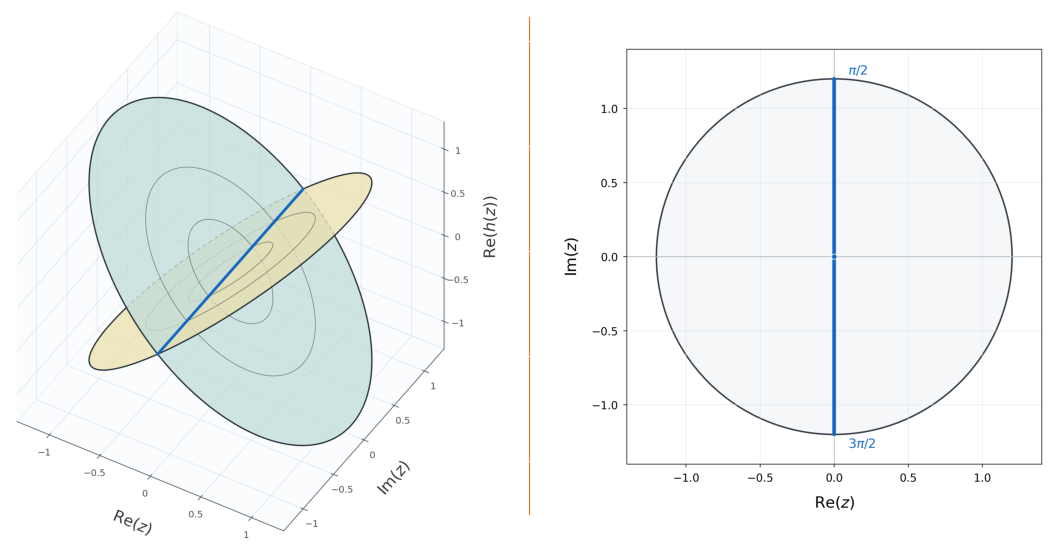
\includegraphics[width=\textwidth]{figures/Numerical_A12_Boutroux.pdf}
		\caption{The local model for a weave edge, as discussed in \Cref{sssec:weave_edge_model}. (Left) The graph of the real part of the multivalued function $h(z)=\pm z$. (Right) The points in the $z$-plane where this real part is univalued.}
		\label{fig:Numerical_A12_Boutroux}
	\end{figure}
\end{center}

\noindent These models are precisely constructed as follows, using the same technique as in \Cref{ssec:Lagrangian_filling_from_AG}. Namely, for each such model we consider a multivalued function $f:\R^2_{x_1,x_2}\lr\R$ and consider the multigraph $\gr(df)\sse(\D^4,\la_\std)$ as in \eqref{eq:graph_df}. In these models $f(x_1,x_2)=\Re(h(z))$ for a multivalued holomorphic function $h:\C_z\lr\C$, where we identify $z=x_1+ix_2$ as in \Cref{lem:complex_curve_real_Lagrangian}.

\subsubsection{Weave edge.}\label{sssec:weave_edge_model} Consider the multivalued function $h(z)$ defined by
\begin{equation}
\boxed{\{h(z)^2=z^2\}}
\end{equation}
\noindent so that the multivalued graph of $h(z)$ is that of the functions $\pm z$. The multigraph of its real part is depicted in \Cref{fig:Numerical_A12_Boutroux} (left), and the locus of points $z\in\C$ where the sheets of $\Re(h(z))$ intersect is drawn in \Cref{fig:Numerical_A12_Boutroux} (right). Geometrically, the Lagrangian surface $\gr(d\Re(h(z)))\sse(\D^4,\la_\std)$ associated to this model consists of two disjoint embedded Lagrangian 2-disks. Note that these two 2-disks are indeed disjoint: the intersection of the two sheets in \Cref{fig:Numerical_A12_Boutroux} (right) disappears in $\gr(d\Re(h(z)))$ because the slopes of the two sheets at the intersections are different, and thus above the locus $\{\Re(z)=0\}$ the differential $dh(z)$ actually has two distinct values as well.

\subsubsection{Trivalent vertex.}\label{sssec:trivalent_model} Consider the multivalued function $h(z)$ defined by
\begin{equation}
\boxed{\{h(z)^2=z^3\}}
\end{equation}
\noindent so that the multivalued graph of $h(z)$ is that of the function $z^{3/2}$. The multigraph of $\Re(h(z))$ is depicted in \Cref{fig:Numerical_D4minus} (left), and the locus of points $z\in\C$ where the sheets of $\Re(h(z))$ intersect is drawn in \Cref{fig:Numerical_D4minus} (right). Such a locus consists of a trivalent vertex, which occurs at $z=0$. There are two points above a point in the $z$-plane which is not in this locus, and one point above the points in this locus. In coordinates, the locus of points in \Cref{fig:Numerical_D4minus} (right), where the graph has at most one value, consists of the union of the three rays $(-1)\R_{\geq0}\cup \left(e^{\pi i/3}\R_{\geq0}\right)\cup \left(e^{-\pi i/3}\R_{\geq0}\right)$.\\

\noindent The projection of the Lagrangian $\gr(d(\Re h(z)))$ onto the $z$-plane, which is identified with the first two coordinates of $\R^4$, is a double branched cover with a unique branch point. Its ramification value is $z=0$, corresponding to the trivalent vertex. In particular the Lagrangian $\gr(d(\Re h(z) ))$ is a 2-plane and it can be verified directly that it is embedded.

\begin{center}
	\begin{figure}[h!]
		\centering		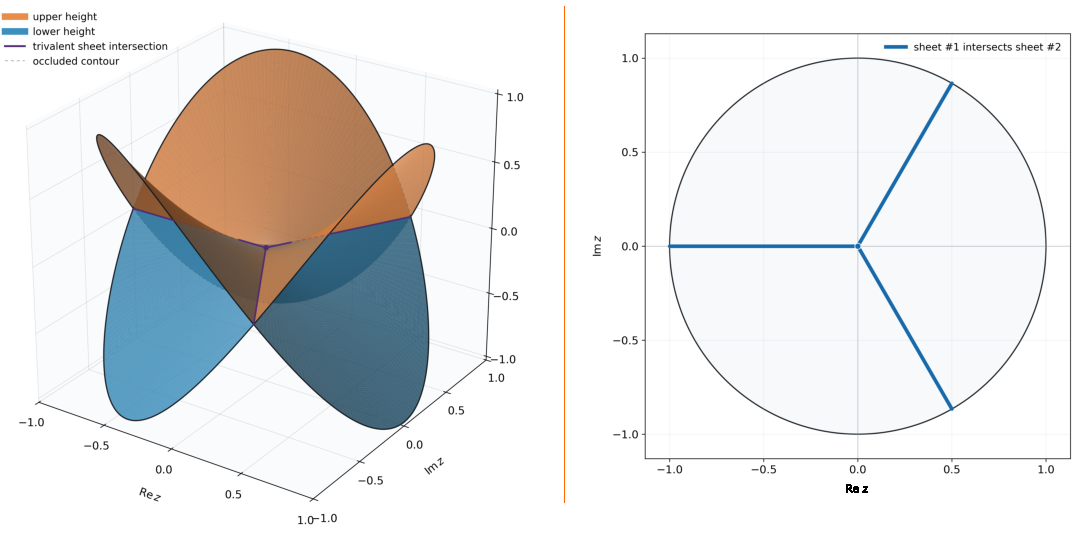
\includegraphics[width=\textwidth]{figures/Numerical_D4minus.pdf}
		\caption{The local model for a trivalent vertex of a weave, as discussed in \Cref{sssec:trivalent_model}. (Left) The graph of the real part of the multivalued function $z^{3/2}$. (Right) The locus of points in the $z$-plane where the function is univalued.}
		\label{fig:Numerical_D4minus}
	\end{figure}
\end{center}

\subsubsection{Hexavalent vertex.}\label{sssec:hexavalent_local_model} Let us consider the multivalued function $h(z)$ defined by
\begin{equation}
\boxed{\{h(z)^3=z^3\}}
\end{equation}
\noindent The multigraph of $\Re(h(z))$ is depicted in \Cref{fig:Numerical_A13minus} (left), and there are three points above a generic point in the $z$-plane. The locus of points $z\in\C$ where the sheets of $\Re(h(z))$ intersect is drawn in \Cref{fig:Numerical_A13minus} (right), where blue indicates that the bottom two sheets intersect and red indicates that the top two sheets intersect. This locus consists of a 6-valent vertex, occurring at $z=0$, and the colors of the edges at the 6-valent vertex alternate between blue and red.\\

\noindent The projection of the Lagrangian $\gr(d(\Re(h(z)))$ onto the $z$-plane is a 3-fold cover, with no branched points. Therefore this Lagrangian consists of 3 disjoint Lagrangian 2-disks, each of them embedded. As a smooth singularity, this $A_1^3$-singularity is equivalent to the origin in the union of the three coordinate planes in $\R^3$, see also \cite[Section 2.2.2]{CasalsZaslow}.

\begin{center}
	\begin{figure}[h!]
		\centering		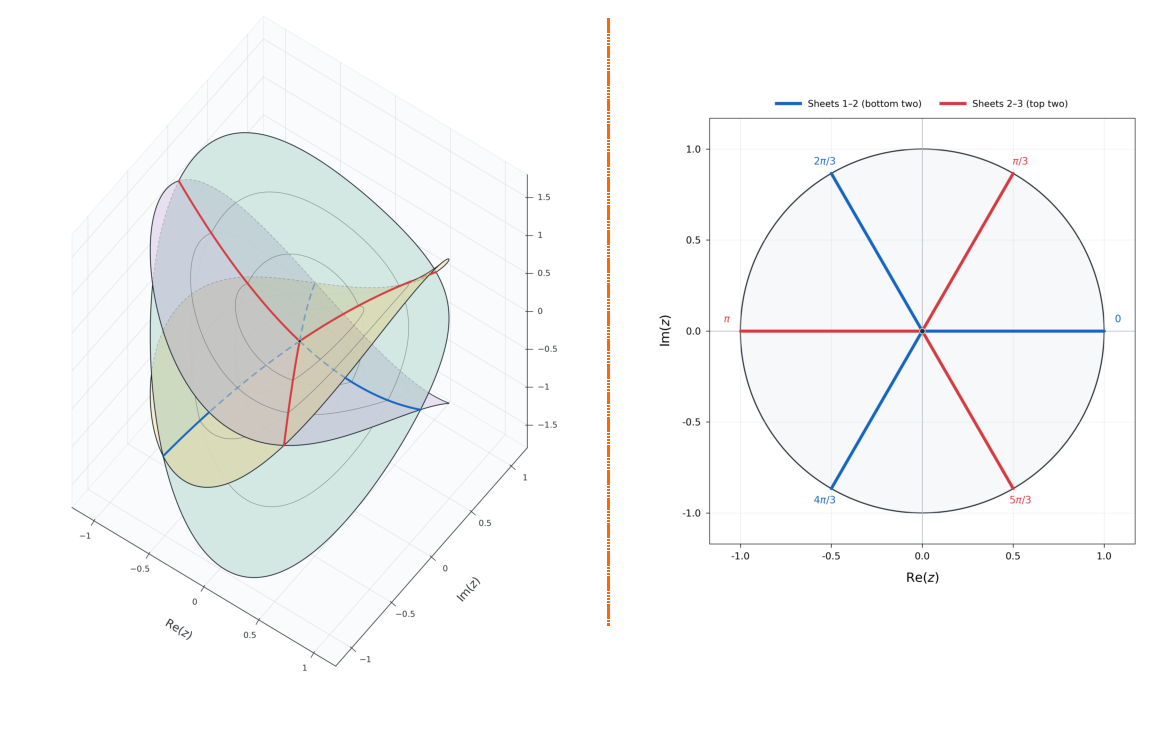
\includegraphics[width=\textwidth]{figures/Numerical_A13minus.pdf}
		\caption{The local model near a hexavalent vertex of a weave, as in \Cref{sssec:hexavalent_local_model}. (Left) The graph of the real part of the multivalued function $\sqrt[3]{z^3}$. (Right) The locus of points in the $z$-plane where the function has fewer than 3 values, with the color indicating which of the different values above a point come together.}
		\label{fig:Numerical_A13minus}
	\end{figure}
\end{center}

\subsubsection{Tetravalent vertex.}\label{sssec:tetravalent_local_model} Let us consider the multivalued function $h(z)$ defined by
\begin{equation}
\boxed{\{\bigl((h(z)+1)^2-z^2\bigr)\bigl((h(z)-1)^2+z^2\bigr)=0\}}
\end{equation}
\noindent The graph of its real part near the origin is depicted in \Cref{fig:Numerical_Tetra_Boutroux} (left). Intuitively, this model consists of two copies of the local model in \Cref{sssec:weave_edge_model}, one on top of the other and the top one rotated by $\pi/2$ radians along the axis perpendicular to the $z$-plane. There are four points above a generic point in the $z$-plane. The locus of points $z\in\C$ where the sheets of $\Re(h(z))$ intersect is drawn in \Cref{fig:Numerical_Tetra_Boutroux} (right), where blue indicates that the bottom two sheets intersect and green indicates that the top two sheets intersect. This locus consists of a 4-valent vertex, occurring at $z=0$, and the colors of the edges at the 4-valent vertices alternate between blue and green.

\begin{center}
	\begin{figure}[h!]
		\centering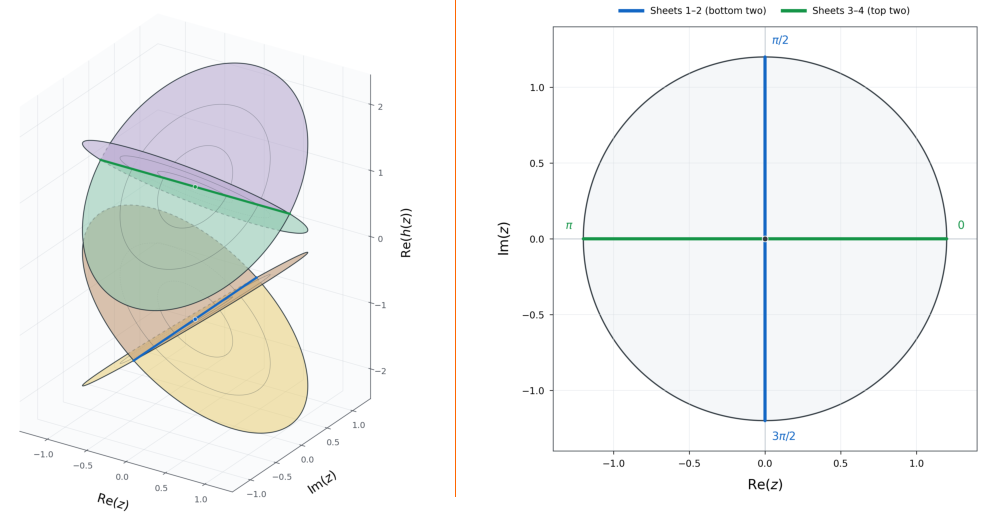
\includegraphics[width=\textwidth]{figures/Numerical_Tetra_Boutroux.pdf}
		\caption{The local model for a tetravalent vertex of a weave, as in \Cref{sssec:tetravalent_local_model}. (Left) The graph of the multivalued function discussed in \Cref{sssec:tetravalent_local_model}. (Right) The locus of points which have fewer than four values above them.}
		\label{fig:Numerical_Tetra_Boutroux}
	\end{figure}
\end{center}

\begin{remark}
These models above can also be parametrized directly with real functions, as was originally done in \cite[Section 2.2]{CasalsZaslow}.\sbs
\end{remark}

\noindent More generally, if we work in $\G=\SL_n$, the Lagrangian local model associated to each piece of the weave is obtained as $\gr(df(z))$ where the graph of $f$ consists of $n$ (almost) parallel sheets with only certain sheets weaving according to the models above. Let us label these sheets $1$ through $n$, bottom to top. Then, these models specifically are as follows:

\begin{enumerate}
    \item For a weave line labeled with $s_j$, we consider $\gr(df(z))$ where the graph of $f$ consists of $n$ (almost) parallel sheets except for sheets $j$ and $j+1$ intersecting according to \Cref{fig:Numerical_A12_Boutroux}. See \Cref{fig:Numerical_ExampleLocalModel} (left) for an example.\\

    \item For a trivalent weave vertex whose edges are labeled with $s_j$, we consider $\gr(df(z))$ where the graph of $f$ consists of $n$ (almost) parallel sheets except for sheets $j$ and $j+1$ intersecting according to \Cref{fig:Numerical_D4minus}. See \Cref{fig:Numerical_ExampleLocalModel} (right) for an example.\\

    \item For a hexavalent weave vertex whose edges are alternately labeled with $s_j$ and $s_{j+1}$, we consider $\gr(df(z))$ where the graph of $f$ consists of $n$ (almost) parallel sheets except for sheets $j,j+1$ and $j+2$ intersecting according to \Cref{fig:Numerical_A13minus}.\\

    
    \item For a tetravalent weave vertex whose edges are alternately labeled with $s_i$ and $s_{k}$, $|i-k|\geq2$, we consider $\gr(df(z))$ where the graph of $f$ consists of $n$ (almost) parallel sheets except for sheets $i,i+1$ and $k,k+1$ intersecting according to \Cref{fig:Numerical_Tetra_Boutroux}.\\
\end{enumerate}

\noindent See \cite[Figure 10]{CasalsZaslow} for another figure illustrating the multigraphs of such local functions.

\begin{center}
	\begin{figure}[h!]
		\centering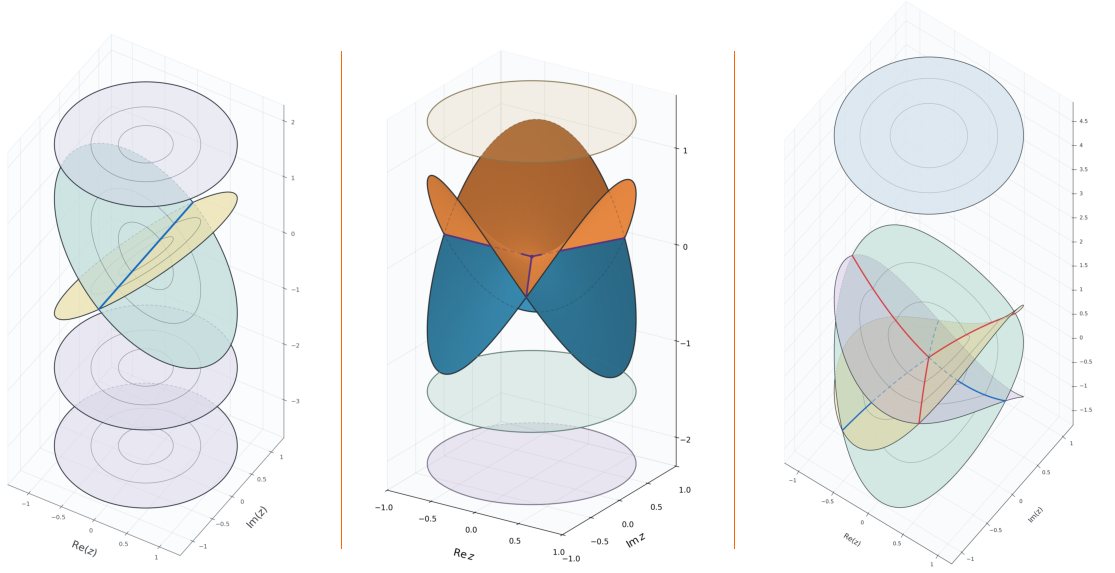
\includegraphics[scale=0.7]{figures/Numerical_ExampleLocalModel.pdf}
		\caption{A way to insert the local models discussed in \Cref{sssec:trivalent_model,sssec:hexavalent_local_model,sssec:tetravalent_local_model} stacking parallel sheets above and below, according to the edge labels of a weave $\w$.}
		\label{fig:Numerical_ExampleLocalModel}
	\end{figure}
\end{center}

%%%%%%%%%%%%%%%%%%%%%%%%%%%%%%%%%%%%%%%%%%%%%%%%%%%%%%%%
%%%%%%%%%%%%%%%%%%%%%%%%%%%%%%%%%%%%%%%%%%%%%%%%%%%%%%%%
%%%%%%%%%%%%%%%%%%%%%%%%%%%%%%%%%%%%%%%%%%%%%%%%%%%%%%%%
\subsection{Lagrangian fillings from a Demazure weave}\label{ssec:Lagrangian_filling_from_weave} Let $\w\sse\Sigma$ be an $n$-weave embedded in a smooth surface $\Sigma$. That is, $\w$ is a graph embedded into $\Sigma$ with only vertices of valence $3,4$ and $6$ whose edges are labeled by simple transpositions $\{s_1,\ldots,s_{n-1}\}$, $s_i\in W(\SL_n)$, cf.~\cite[Section 2.3]{CasalsZaslow}. If $\D^2\sse\Sigma$ is a 2-disk such that $\w\cap\D^2$ is a neighborhood of a weave edge or a weave vertex in $\w$, we constructed in \Cref{ssec:Lagrangian_filling_from_weave_local_models} a corresponding local exact Lagrangian surface $L\sse T^*\D^2$ as the multigraph of a differential of a function. This construction is globalized as follows:

\begin{fdef}[Lagrangian filling of a Demazure weave]\label{def:Lagrangian_from_weave} Let $\w\sse\Sigma$ be a $n$-weave embedded in a smooth surface $\Sigma$. By definition, the exact Lagrangian surface $L_\w\sse (T^*\Sigma,\la_\std)$ is the Lagrangian surface constructed as follows:

\begin{enumerate}
    \item Cover $\Sigma$ by a finite collection of 2-disks $\D^2_i$ such that $\w\cap\D^2_i$ consists exactly of one of the four local models of a weave, i.e.~a weave line, or a vertex of valence either 3, 4 or 6, labeled with the corresponding simple transpositions.\\

    \item On each given such 2-disk $\D^2_i$, we choose a model of the corresponding local Lagrangian surface so that for different 2-disks $\D^2_i$ and $\D^2_j$ the models coincide above the intersection $\D^2_i\cap\D^2_j$.
\end{enumerate}
The result from gluing such local Lagrangian surfaces defines a Lagrangian surface $L_\w\sse (T^*\Sigma,\la_\std)$.\sbs
\end{fdef}
\vspace{0.2cm}
\noindent In \Cref{def:Lagrangian_from_weave} we have used the notation $(T^*\Sigma,\la_\std)$ to indicate the cotangent bundle of $\Sigma$, as an exact symplectic 4-manifold, endowed with the canonical Liouville form $\la_\std$. There are choices in \Cref{def:Lagrangian_from_weave}: the cover of $\Sigma$ by the 2-disks and the corresponding model for the local Lagrangian surface above each such 2-disk. The Hamiltonian isotopy type of $L_\w$ is independent of such choices, and the latter choices exist even when requiring the local models to coincide at their intersections. A few comments on \Cref{def:Lagrangian_from_weave}:

\begin{enumerate}
    \item The Lagrangian surface $L_\w\sse (T^*\Sigma,\la_\std)$ is exact and orientable by construction. Intuitively, when we glue the local models over disks in $\Sigma$ from \Cref{ssec:Lagrangian_filling_from_weave_local_models} together: each local model is given as $\gr(df_i)$ for some multivalued function $f_i:\D^2\lr\R$ and it is possible to glue those multivalued functions as well to obtain a global multivalued function $F:\Sigma\lr\R$. The result is that $L_\w$ is also of the form $\gr(dF)\sse T^*\Sigma$ for some multivalued function $F:\Sigma\lr\R$. \footnote{Rigorously, it is the Lagrangian projection of a Legendrian surface, and thus exact.}\\

    \noindent Two examples of the multigraphs of such global multivalued $F:\D^2\lr\R$ in \Cref{def:Lagrangian_from_weave} are depicted in \Cref{fig:Numerical_Trefoil_2weave} and \Cref{fig:Numerical_34_3weave}, with the corresponding weaves $\w$ depicted to their right.\\

    \item The Lagrangian surface $L_\w\sse (T^*\Sigma,\la_\std)$ is immersed, but typically not embedded. For a Demazure weave $\w:\beta\lr\delta(\beta)$, there is a way to choose and glue the local models so as to have $L_\w\sse (T^*\Sigma,\la_\std)$ be embedded, see e.g.~\cite[Section 7.1]{casals2025spectralnetworksbettilagrangians}. The Hamiltonian isotopy class of $L_\w\sse (T^*\Sigma,\la_\std)$ is independent of such choices, cf.~\cite[Section 2]{casals2022conjugate}. Thus, given a Demazure weave $\w\sse\Sigma$, there is a uniquely well-defined embedded exact Lagrangian $L_\w\sse (T^*\Sigma,\la_\std)$, up to Hamiltonian isotopy.\\
\end{enumerate}

\noindent For specificity, we will focus on Lagrangian fillings $L_\w\sse(\D^4,\la_\std)$ associated to a Demazure weave $\w\sse\D^2$. Thus we set $\Sigma=\D^2$ and $\w:\beta\lr\delta(\beta)$ Demazure in \Cref{def:Lagrangian_from_weave} onwards. In this case, $L_\w$ is a Lagrangian filling of
$$\boxed{\dd L_\w=\La_\beta}$$
with $\La_\beta$ as in \Cref{def:Legendrian_from_braid}.

\begin{remark}
In general, even if $\w$ is a Demazure weave on the disk $\Sigma=\D^2$, the embedded exact Lagrangian $L_\w\sse(\D^4,\la_\std)$ cannot be obtained from an algebraic curve via \Cref{lem:complex_curve_real_Lagrangian}. To start, the Legendrian link $\La_\beta$ at the boundary might not even be an algebraic link. Note also that, in contrast to \Cref{lem:complex_curve_real_Lagrangian} and \Cref{ex:special_fillings}, \Cref{def:Lagrangian_from_weave} is such that $L_\w$ is automatically exact, or at least it is relatively simple to prove that. Thus, helpfully, there is no need for the finer tuning in \Cref{lem:complex_curve_real_Lagrangian} and \Cref{ex:special_fillings} to have certain periods vanish and, at least in this regard, manipulating $L_\w$ is much closer to manipulating smooth surfaces in geometric topology than it is to manipulating algebraic curves in complex algebraic geometry.\sbs
\end{remark}

%%%%%%%%%%%%%%%%%%%%%%%%%%%%%%%%%%%%%%%%%%%%%%%%%%%%%%%%
%%%%%%%%%%%%%%%%%%%%%%%%%%%%%%%%%%%%%%%%%%%%%%%%%%%%%%%%
%%%%%%%%%%%%%%%%%%%%%%%%%%%%%%%%%%%%%%%%%%%%%%%%%%%%%%%%
\subsection{Smooth topology of Lagrangian fillings $L_\w$}\label{ssec:smooth_topology_Lagrangian_filling_from_weave} The smooth topology of the Lagrangian fillings constructed in \Cref{def:Lagrangian_from_weave} can be determined as in \Cref{rmk:topology_Lagrangian_filling}. The key fact is that the restriction to $L_\w$ of the projection $\D^4\lr\R^2_{x_1,x_2}$ onto the first two coordinates is a simple $n$-fold branched cover
\begin{equation}\label{eq:branched_cover_map}
\pi:L_\w\lr\R^2_{x_1,x_2}
\end{equation}
\noindent branched over the trivalent vertices of $\w$. The two sheets where the branch point occurs in $L_\w$ over a given trivalent vertex are the $i$th and $(i+1)$st sheets if the weave edges of that trivalent vertex are labeled by $s_i$, cf.~\Cref{fig:Numerical_ExampleLocalModel} (center). In a sense:
\begin{center}
  \fbox{%
    \begin{tabular}{l}
      \itshape A weave $\w$ is a choice of branch cuts for the branched cover $L_\w\lr\R^2_{x_1,x_2}$ which is particularly suited to \\
      \itshape the contact and symplectic topology of $L_\w$ and its resulting Floer-theoretic and sheaf-theoretic invariants.
    \end{tabular}%
  }
\end{center}
\vspace{0.2cm}
\noindent This viewpoint above is particularly useful when studying both additive and monoidal categorifications of Demazure weaves. Geometrically, it also allows for the construction of Lagrangian skeleta in certain 6-dimensional exact symplectic manifolds whose Fukaya categories provide such additive categorifications, cf.~\cite{CasalsChrist}. We emphasize that it is an excessive choice, in that many more cuts are considered than minimally needed to trivialize the branched cover \eqref{eq:branched_cover_map}. That said, as motivated by \Cref{ssec:Lagrangian_filling_from_AG} and the number of new results one can prove with weaves through this viewpoint, it is certainly a useful choice of branch cuts.\\

The properties of the branched cover map \eqref{eq:branched_cover_map} imply the following result:

\begin{lemma}\label{lem:smooth_topology_weave_fillings}
Let $\beta\in\brn$ be a positive braid word and $\w:\beta\lr\delta(\beta)$ a Demazure weave. Then:\\

\begin{enumerate}[label=$(\roman*)$]
    \item The number of components of the Legendrian link $\La_\beta$ is equal to the number of cycles in the cycle decomposition of the permutation underlying $\beta\delta(\beta)$.\\

    \item The Euler characteristic of $L_\w$ is $\chi(L_\w)=n-\#(\mbox{trivalent vertices of }\w)$.\\

    \item Consider the relative first homology $\operatorname{H}_1(L_\w,\tt,\Z)$, where $\tt$ is the set of basepoints of $\dd L_\w=\La_\beta$, one per strand. Then
    $$\operatorname{rk}\left(\operatorname{H}_1(L_\w,\tt,\Z)\right)=b_1(L_\w)+n-|\pi_0(L_\w)|.$$
    \sbs
\end{enumerate}
\end{lemma}

\noindent Since $L_\w$ is orientable, if it is connected, then its number of boundary components, supplied by \Cref{lem:smooth_topology_weave_fillings}.(i), and its Euler characteristic, supplied by \Cref{lem:smooth_topology_weave_fillings}.(ii), uniquely determine the abstract diffeomorphism type of $L_\w$, as a smooth surface. As above, from now on, let us endow $\La_\beta$ with one marked point per strand, located to the right of all the crossings of $\beta$, cf.~the $t_{r,i}$ basepoints in \cite[Figure 23]{CasalsNg22}, $i\in[1,n]$, or \cite[Figure 2 (left)]{casals2026vanishinghigherlegendrianhomology}. Let $\mathfrak{t}$ be such set of marked points.

%%%%%%%%%%%%%%%%%%%%%%%%%%%%%%%%%%%%%%%%%%%%%%%%%%%%%%%%
%%%%%%%%%%%%%%%%%%%%%%%%%%%%%%%%%%%%%%%%%%%%%%%%%%%%%%%%
\subsubsection{The $\SX$ and $\SA$-lattices}\label{sssec:X_lattice} Following the viewpoint of \cite{FG2006,FG09}, cluster seeds can be interpreted as bases of a certain lattice with additional data, see e.g.~\cite[Appendix A]{GHKK18}. In the context of Demazure weaves $\w$, the lattice $M$, which corresponds to the cluster $\SX$-variety, can be interpreted in terms of the Lagrangian filling $L_\w$. Specifically, given a Demazure weave $\w:\beta\to\delta(\beta)$, the $\SX$-lattices are:
$$M:=\hH_1(L_\w,\tt;\Z)\qquad\mbox{ and }\qquad M_{un}:=\hH_1(L_\w;\Z),$$
\noindent where $\hH_1(L_\w,\tt;\Z)$ denotes the first integral relative homology group of the relative pair $(L_\w,\tt)$, with $\tt\sse\dd L_\w$ denoting the set of marked points in $\dd L_\w=\La_\b$. The natural inclusion of the absolute integral homology group $\hH_1(L_\w;\Z)\hookrightarrow \hH_1(L_\w,\tt;\Z)$ provides an inclusion of the unfrozen lattice $M_{un}$, a.k.a.~the mutable sublattice, inside of $M$.

\begin{center}
	\begin{figure}[h!]
		\centering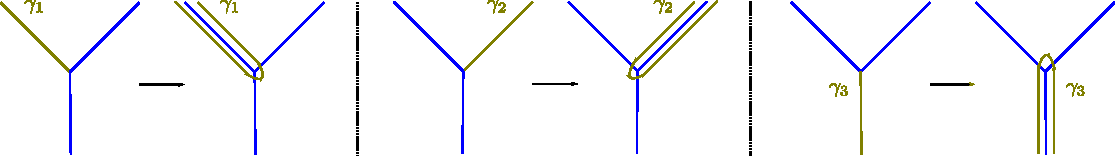
\includegraphics[width=\textwidth]{figures/Cycles_Trivalent_Perturb.pdf}
		\caption{Perturbations of the 1-cycles associated to a weave cycle $\g_i$, $i\in[1,3]$. On the left of each of these three situations, the 1-cycle $\g_i$ projects directly to an edge of the weave $\w$. On the right, the 1-cycle has been deformed in $L_\w$ so that its projection is an embedded relative cycle. These perturbations are necessary in order to geometrically compute the intersections between weave cycles.}
		\label{fig:Cycles_Trivalent_Perturb}
	\end{figure}
\end{center}

\noindent Dually, there is also a construction for the $\SA$-lattice:
$$N:=\hH_1(L_\w\setminus \tt,\La_\beta\setminus \tt;\Z)$$
and its corresponding mutable sublattice. This $\SA$-lattice above appears naturally when studying the long exact sequence of the triple $(L_\w,\dd L_\w,\tt)$, cf.~\cite[Section 3.10]{CasalsWeng22}, as $\dd L_\w=\La_\beta$. Note that there is a non-degenerate intersection pairing between such $M$ and $N$, providing the appropriate duality.\\

In \Cref{sssec:Lusztigcycles} we introduced the Lusztig cycles over a Demazure weave $\w:\beta\to\delta(\beta)$, cf.~\Cref{def:Lusztig_cycles}. These weave cycles have key geometric meaning in the context of contact and symplectic topology. At the most basic level there is the following construction. For each Lusztig cycle $\g$ of $\w$, we can construct an element $[\gamma]\in \hH_1(L_\w,\tt;\Z)$ by drawing certain curves in the plane $\R^2_{x_1,x_2}$ where $\w$ is depicted and lifting them through the branched cover $L_\w\lr \R^2_{x_1,x_2}$. This is explained in \cite[Section 7.4]{CGGLSS25} and \cite[Section 2.4]{CasalsZaslow}. Intuitively, given a weave edge labeled by $s_i$, we can consider the two arcs above the weave edge at the sheets $i$ and $(i+1)$st. The interesting fact about the combinatorics of Lusztig cycles is that these arcs glue well at the trivalent and hexavalent vertices.

\begin{center}
	\begin{figure}[h!]
		\centering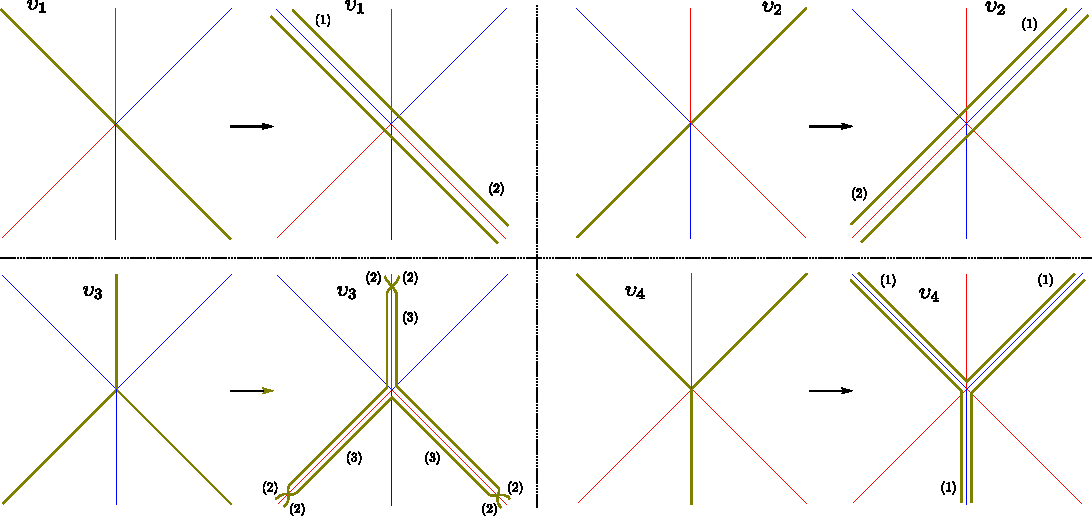
\includegraphics[width=\textwidth]{figures/Cycles_Hexavalent_Perturb2.pdf}
		\caption{Perturbations of a few Lusztig cycles near the hexavalent vertex of a weave.}
		\label{fig:Cycles_Hexavalent_Perturb2}
	\end{figure}
\end{center}

A way to visually understand how such gluing occurs is to perturb these arcs slightly off so they do not live on top of the weave edge under \eqref{eq:branched_cover_map}, and then directly draw their behavior via their images in $\R^2_{x_1,x_2}$, lifting those curves in $\R^2_{x_1,x_2}$ to the appropriate sheets. \Cref{fig:Cycles_Trivalent_Perturb} depicts an instance of this near a trivalent vertex with label $s_i$, where the only two sheets that are relevant are the $i$ and $(i+1)$st sheets. Similarly, \Cref{fig:Cycles_Hexavalent_Perturb2} depicts an example of this near a hexavalent vertex. The tropical Lusztig rules near trivalent and hexavalent vertices are explained in terms of these curves in \Cref{fig:Cycles_Lusztig2}.

\begin{remark}
In the case of the frozen Lusztig cycles, one needs to adjust the ends so as to lie in $\tt$: such adjustment is possible but different choices lead to interesting quasi-cluster equivalences, cf.~\cite[Section 5.5]{CGGLSS25} and \cite{casals2023demazureweavesreducedplabic}.\sbs
\end{remark}

\noindent A similar construction applies to the dual Lusztig cycles from \Cref{def:dual_Lusztig_cycles}. From a dual Lusztig cycle $\rho$ of $\w$ one can similarly construct an element $[\rho]\in\hH_1(L\setminus\tt,\La\setminus\tt;\Z)$ . Given the Lusztig cycles $\{\g_i\}$ and their duals $\{\rho_i\}$, their corresponding homology classes $\{[\g_i]\}$ and $\{[\rho_i]\}$ are Poincar\'e dual to each other, under the non-degenerate intersection pairing between $\hH_1(L_\w,\tt;\Z)$ and $\hH_1(L_\w\setminus \tt,\dd L_\w\setminus \tt;\Z)$.

\begin{center}
	\begin{figure}[h!]
		\centering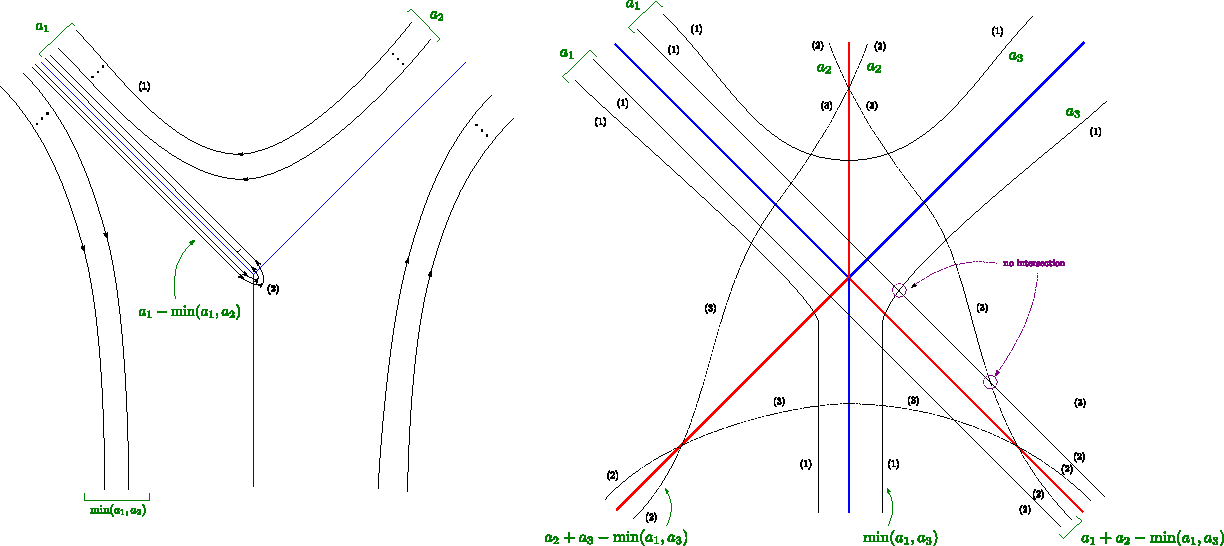
\includegraphics[width=\textwidth]{figures/Cycles_Lusztig2.pdf}
		\caption{The geometric models explaining how the tropical propagation rules for Lusztig cycles in $\w$ arise when intersecting relative $1$-cycles in the surface $L_\w$.}
		\label{fig:Cycles_Lusztig2}
	\end{figure}
\end{center}

\noindent Since the topology of $L_\w$ is essentially generated by the branched points of \eqref{eq:branched_cover_map}, and thus the trivalent vertices of $\w$ from a combinatorial viewpoint, it can be deduced that the Lusztig cycles of $\w$ provide a basis for the lattice. We summarize these properties in the following:

\begin{lemma}\label{lem:lustzig_cycles_basis}
Let $\w:\beta\to\delta(\beta)$ be a Demazure weave. Then the following hold:

\begin{enumerate}[label=$(\roman*)$]
    \item The homology classes associated to the mutable Lusztig cycles of $\w$ form a basis of the mutable $\SX$-lattice $\hH_1(L_\w;\Z)$. Similarly, the homology classes $\{[\g_i]\}$ associated to the Lusztig cycles $\{\g_i\}$ of $\w$ form a basis of the $\SX$-lattice $\hH_1(L_\w,\tt;\Z)$.\\

    \item The homology classes $\{[\rho_i]\}$  associated to the dual Lusztig cycles $\{\rho_i\}$ of $\w$ form a basis of the $\SA$-lattice $\hH_1(L_\w\setminus \tt,\La_\beta\setminus\tt;\Z)$.\\

    \item Let $\eta_1$ be a Lusztig cycle or a dual Lusztig cycle, and let $\eta_2$ another such cycle. Then
    $$\langle \eta_1,\eta_2\rangle_\w=\langle[\eta_1],[\eta_2]\rangle$$
    where the left hand side is the weave intersection form, as in \Cref{ssec:intersection_cycles}, and the right hand side is the algebraic intersection product in homology, induced by the cap product.\\
\end{enumerate}
\noindent In particular, the two bases $\{[\g_i]\}$  and $\{[\rho_i]\}$ are dual bases under the non-degenerate intersection pairing between $\hH_1(L_\w,\tt;\Z)$ and $\hH_1(L_\w\setminus \tt,\La_\beta\setminus\tt;\Z)$.\sbs
\end{lemma}

\noindent Note that, technically, the algebraic intersection pairing of two homology classes in $\hH_1(L_\w,\tt;\Z)$ requires a boundary push-off (or an order convention). We are implicitly making such a choice when computing in $\hH_1(L_\w,\tt;\Z)$, see \cite[Section 3.2]{CGGJ24}.

%%%%%%%%%%%%%%%%%%%%%%%%%%%%%%%%%%%%%%%%%%%%%%%%%%%%%%%%
%%%%%%%%%%%%%%%%%%%%%%%%%%%%%%%%%%%%%%%%%%%%%%%%%%%%%%%%
%%%%%%%%%%%%%%%%%%%%%%%%%%%%%%%%%%%%%%%%%%%%%%%%%%%%%%%%
\subsection{Demazure weaves and Lagrangian cobordisms}\label{ssec:Lagrangian_coboridsms} In \Cref{sec:weaves_braid_varieties}, \Cref{sec:braid_variety_cluster} and \Cref{sec:Reeb_variables} we studied the connection of a Demazure weave $\w:\beta\to\delta(\beta)$ to the braid variety $X(\beta)$ by scanning the weave $\w$ top-to-bottom, cf.~\Cref{ssec:weave_tori_braid_varieties}. Specifically, given a vertex $v\in\w$ we can consider the horizontal slices $h_\pm$ above and below $v$ and the corresponding positive braid words $\beta_{\pm}$, as in \Cref{fig:BraidVariety_DiagramMoves2} and \Cref{fig:BraidVariety_Trivalent2}:
\begin{enumerate}
    \item At hexavalent and tetravalent vertices, \Cref{lem:braid_invariance} provides isomorphisms
    \begin{equation}\label{eq:cobordism_maps_braid_varieties}R3:X(\beta_-)\stackrel{\simeq}{\lr} X(\beta_+),\quad C:X(\beta_-)\stackrel{\simeq}{\lr} X(\beta_+)
    \end{equation}

    \item At a trivalent vertex, \Cref{lem:braidvarieties_trivalent} provides an open embedding \begin{equation}\label{eq:cobordism_maps_braid_varieties2}
        \iota_v:X(\beta_-)\times\bG_m\hookrightarrow X(\beta_+).
    \end{equation}
 \end{enumerate}

\noindent The Lagrangian local models for these vertices, as presented in \Cref{ssec:Lagrangian_filling_from_weave_local_models}, actually yield Lagrangian cobordisms $L_v$ from $\La_{\beta_-}$ to $\La_{\beta_+}$, $\La_{\beta_-}$ at the concave end and $\La_{\beta_+}$ at the convex end. See for instance \cite[Section 6]{EtnyreNg22_Survey} for a survey on Lagrangian cobordisms. These Lagrangian cobordisms $L_v$ occur in the symplectization of $(\R^3,\xi_\std)$, and are exact and embedded. In particular, each such Lagrangian cobordism $L_v$ induces a dg algebra map
\begin{equation}\label{eq:cobordism_map}
\varepsilon_{L_v}:\mathbb{A}(\La_{\beta_+})\lr \mathbb{A}(\La_{\beta_-})\otimes_{\Z[C_{-*}(\Omega \La_{\beta_-})]} \Z[C_{-*}(\Omega L_v)]
\end{equation}
as in \cite[Theorem 1.6]{EHK} or \cite[Theorem 6.3]{EtnyreNg22_Survey}. See also \cite{LiCobordism1,li2024lagrangiancobordismfunctormicrolocal}.

\begin{example} The maps \Cref{eq:cobordism_map} are a refinement of \Cref{eq:augmentation_map_filling}, which corresponds to the case where $\La_{\beta_-}=\emptyset$ is empty. Indeed, a Lagrangian filling is a Lagrangian cobordism with empty concave (bottom) end: \Cref{prop:torus_from_filling} encodes precisely \eqref{eq:cobordism_map} where $\mathbb{A}(\La_{\beta_-})\cong \Z$, generated by the unit (the empty word on Reeb chords), and we identify
$$\hH_0(C_{-*}(\Omega L;\Z))^{ab}\cong\Z[\pi_1(L)]^{ab}\cong\Z[\hH_1(L;\Z)]\cong\Z[s_1^{\pm1},\ldots,s^{\pm1}_{b_1(L)}],$$
as $L$ is a punctured smooth surface, cf.~\cite{EkholmLekili2023}.\sbs    
\end{example}
\noindent In particular, $\varepsilon_{L_v}$ induces a morphism between the $\mbox{H}_0$ of their abelianizations. After applying $\Spec$ to $\hH_0$ of the abelianization of \eqref{eq:cobordism_map} and base changing to $k$, we obtain:
\begin{enumerate}
    \item At a hexavalent or tetravalent vertex $v\in\w$, the Lagrangian cobordism $L_v$ is the Lagrangian concordance given by the trace of a Legendrian Reidemeister III move (\Cref{fig:Front_Arc_Cusp_Crossing_R3_Reidemeister}) or the Legendrian isotopy given by a commutation of distant crossings, respectively. The Floer theoretic map \eqref{eq:cobordism_map} provides isomorphisms
    \begin{equation}\label{eq:Floer_maps_iso}\Spec\mbox{H}_0(\mathbb{A}^{ab}(\La_{\beta_-}))\stackrel{\simeq}{\lr} \Spec\mbox{H}_0(\mathbb{A}^{ab}(\La_{\beta_+})),\quad \Spec\mbox{H}_0(\mathbb{A}^{ab}(\La_{\beta_-}))\stackrel{\simeq}{\lr} \Spec\mbox{H}_0(\mathbb{A}^{ab}(\La_{\beta_+}))
    \end{equation}

    \item At a trivalent vertex, \eqref{eq:cobordism_map} provides an open embedding \begin{equation}\label{eq:Floer_inclusion_trivalent}
        \Spec\mbox{H}_0(\mathbb{A}^{ab}(\La_{\beta_-}))\times\bG_m\hookrightarrow \Spec\mbox{H}_0(\mathbb{A}^{ab}(\La_{\beta_+})),
    \end{equation}
    where the $\bG_m$-factor can be geometrically identified as $\bG_m\cong \Spec k[H_1(L_\w,\La_{\beta_-};\Z)]\cong \Spec k[\tau^{\pm1}]$ is generated by the relative homology class $\tau$ of the stable manifold of the unique critical point of the saddle cobordism $L_\w$, where $\w$ has a unique trivalent vertex.
 \end{enumerate}

\noindent  Here is a refinement of \Cref{prop:torus_from_filling}, in the form of a horizontal slice decomposition, in the context of Lagrangian cobordisms associated to weave vertices:

\begin{lemma}[Floer theory morphisms induce weave morphisms]\label{lem:floer_morphisms_weave_morphisms}
Let us consider the identification $X(\beta)\cong \Spec \mbox{H}_0(\mathbb{A}^{ab}(\La_{\beta}))$ of \Cref{thm:braid_varieties_from_Legendrian}.(i), see also \Cref{eq:braid_variety_dga2}. Then the weave morphisms \eqref{eq:cobordism_maps_braid_varieties} and \eqref{eq:cobordism_maps_braid_varieties2} coincide with the Floer-theoretically induced morphisms \eqref{eq:Floer_maps_iso} and \eqref{eq:Floer_inclusion_trivalent}, respectively.\sbs
\end{lemma}

\noindent \Cref{lem:floer_morphisms_weave_morphisms} follows from the description of the Floer-theoretic maps in \cite[Section 5]{CasalsNg22}. There is a result similar to \Cref{lem:floer_morphisms_weave_morphisms} for the sheaf-theoretic induced morphisms, using the other identifications in \Cref{thm:braid_varieties_from_Legendrian}. A few comments are in order:

\begin{enumerate}
    \item In the diagrammatic calculus of Demazure weave, we prominently used the Reeb coordinates, as discussed in \Cref{sec:Reeb_variables}. These variables coincide with the Floer-theoretic variables that keep track of the degree 0 Reeb chords associated to the $(-1)$-closure of $\beta\delta(\beta)$. Specifically, for such fronts, there are Reeb chords only in degrees 0 and 1, which generate the Legendrian dg algebra $\mathbb{A}(\La_{\beta})$. The Reeb chords of degree 0 correspond to the crossings of $\beta\delta(\beta)$. Intuitively, we can think of the degree 0 Reeb chords as generators and the differentials of the degree 1 Reeb chords as relations among them, cf.~\cite[Section 5]{CasalsNg22} and \cite[Corollary 1.1]{casals2026vanishinghigherlegendrianhomology}. Via the identification
    $$X(\beta)\cong \Spec \mbox{H}_0(\mathbb{A}^{ab}(\La_{\beta}))$$
    of \Cref{thm:braid_varieties_from_Legendrian}.(i), this description precisely leads to the Reeb $z$-coordinates for $X(\beta)$ and the corresponding equations from \Cref{lem:equations_braidvar}.\footnote{To be precise, from a Floer-theoretic viewpoint, there are also $z$-coordinates associated to the degree 0 Reeb chords from the crossings of $\delta(\beta)$, but the differentials of the degree 1 Reeb chords can be used to express those in terms of the $z$-coordinates of the degree 0 Reeb chords associated to the crossings of $\beta$.}\\

    \item The torus $\T$-action on $X(\beta)$ described in \Cref{sssec:braid_variety_further_symmetries} also has a symplectic interpretation. Namely, it corresponds to the $\T$-action induced by link automorphisms on the Legendrian dg algebra, cf.~\cite[Section 3.2]{CasalsNg22}. In brief, these are automorphisms induced by carrying around the basepoints of a Legendrian link around their corresponding components. In our case, the basepoints are all located to the right of all the degree 0 Reeb chords, i.e.~of all the crossings of $\beta\delta(\beta)$. Moving them past the crossings of $\beta\delta(\beta)$ and keeping track of their action on the corresponding degree 0 Reeb chords, using \cite[Section 4.1.1]{CasalsNg22}, leads to a Floer-theoretic proof of the formula \Cref{lem:torusaction_coordinates}.
\end{enumerate}
%%%%%%%%%%%%%%%%%%%%%%%%%%%%%%%%%%%%%%%%%%%%%%%%%%%%%%%%
%%%%%%%%%%%%%%%%%%%%%%%%%%%%%%%%%%%%%%%%%%%%%%%%%%%%%%%%
%%%%%%%%%%%%%%%%%%%%%%%%%%%%%%%%%%%%%%%%%%%%%%%%%%%%%%%%
\begin{remark} It should be mentioned that, in line with \Cref{ssec:Demazure_weaves_from_combinatorics}, a first connection between the combinatorics of reduced plabic graphs, and Lagrangian fillings was studied in \cite{STWZ19}. Such Lagrangian enhancements of the conjugate surfaces from \cite{GonKen13} illustrated some of the advantages of using the microlocal theory of sheaves in relation to cluster structures, especially the use of microlocal parallel transport. Note also that there exists a hybrid calculus, developed in \cite{casals2022conjugate}, combining (and transitioning between) these Lagrangian conjugate surfaces and weaves.\sbs
\end{remark}